% Starter deck -- edit me, then `make` (-> talk.pdf).
% Every feature of the theme is demonstrated in examples/template.tex.
\documentclass[aspectratio=169]{beamer}

% brand=ncar|ucar|ncarucar   title=dark|light   footer=minimal|full
\usetheme[brand=ncar, title=dark]{NCAR}

\usepackage{booktabs}
\usepackage{listings}

\title{Talk Title Goes Here}
\subtitle{An optional subtitle}
\author{Your Name}
\institute{Your Title, Your Lab, NSF NCAR}
\date{\today}
\titlegraphic{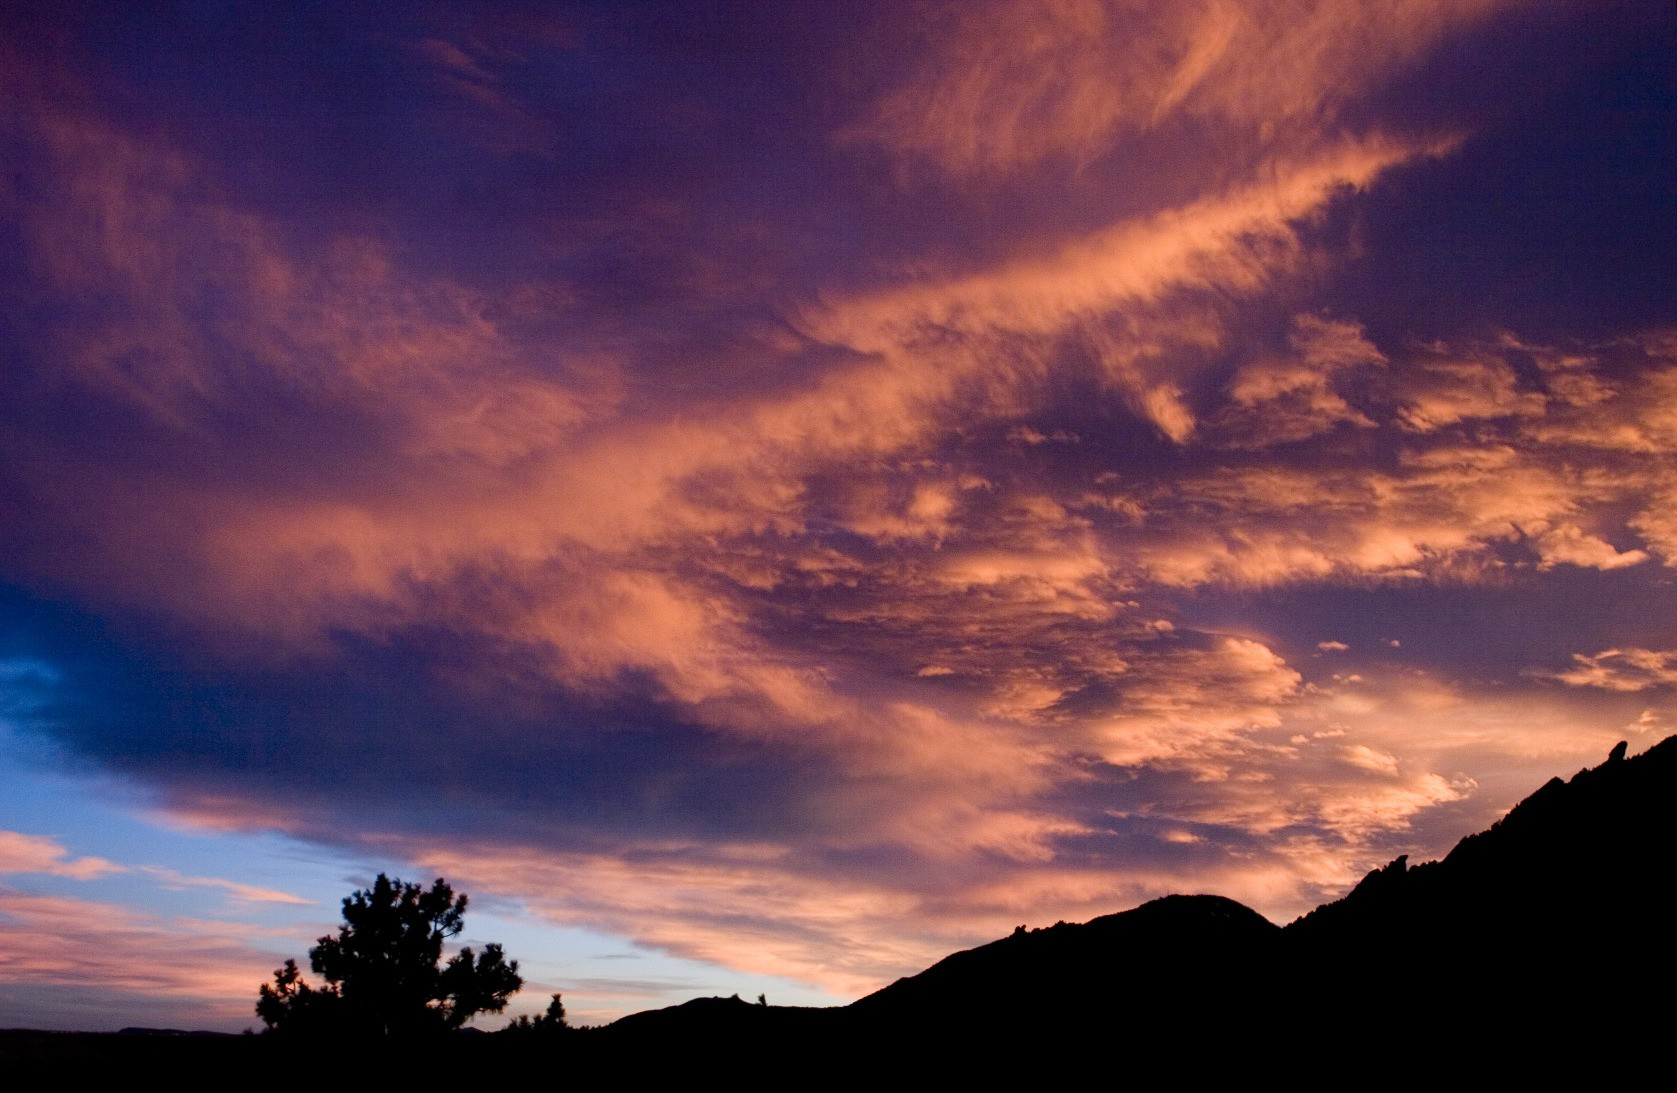
\includegraphics{images/wallpaper/mesa_lab_sunset.jpg}} % optional
\titlefineprint{This material is based upon work supported by the NSF National
  Center for Atmospheric Research, a major facility sponsored by the
  U.S.~National Science Foundation.}

\begin{document}

\begin{frame}[plain,noframenumbering]
  \titlepage
\end{frame}

\section{Introduction}

\begin{frame}{A Content Slide}
  \begin{itemize}
  \item Make a point
    \begin{itemize}
    \item and support it
    \end{itemize}
  \item Highlight \alert{one key idea}
  \end{itemize}
  \begin{block}{A block}
    Blocks, example blocks, and alert blocks are all branded.
  \end{block}
\end{frame}

\begin{frame}[ncarbg=images/wallpaper/mesa_lab.jpg]{A Photo Slide}
  \vfill
  \begin{block}{Blocks turn translucent on photos}
    \texttt{\textbackslash begin\{frame\}[ncarbg=photo.jpg]}
  \end{block}
\end{frame}

\section{Details}

\begin{frame}[fragile]{Code}
\begin{lstlisting}[language=bash]
#!/bin/bash
#PBS -A <project>
#PBS -l select=1:ncpus=128
mpiexec ./my_model
\end{lstlisting}
\end{frame}

\ncarclosingframe{Thank you!}{%
  Questions?\par\medskip
  \textbf{Your Name}\\ \texttt{you@ucar.edu}}

\end{document}
